\section{The Body}

\subsection{Shorter Not Equal to Faster}

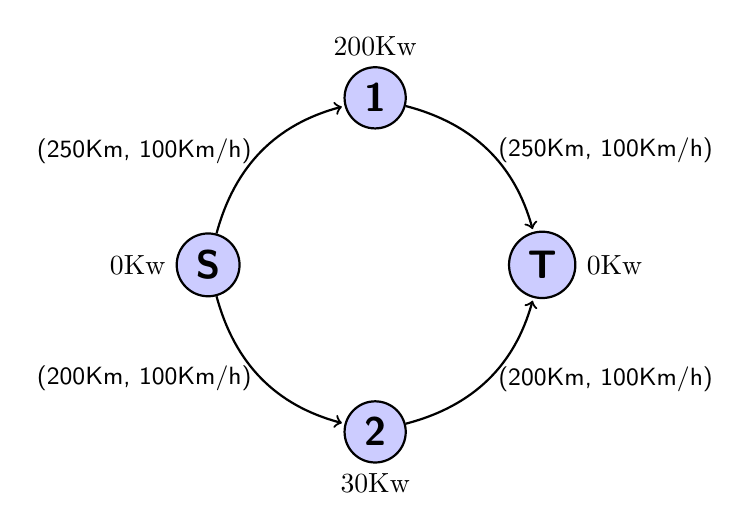
\begin{tikzpicture}[->,->,shorten >=1pt,auto,node distance=3cm,
  thick,main node/.style={circle,fill=blue!20,draw,font=\sffamily\Large\bfseries}]
%1
  \node[main node] (1) {1};
  \node[above] at (1.north) {200Kw};
%2 
 \node[main node] (2) [below left of=1] {S};
  \node[left] at (2.west) {0Kw};
%3 
 \node[main node] (3) [below right of=2] {2};
  \node[below] at (3.south) {30Kw};
%4 
 \node[main node] (4) [below right of=1] {T};
  \node[right] at (4.east) {0Kw};
%paths
  \path[every node/.style={font=\sffamily\small}]
    (1)
	  edge [bend left] node[right] {(250Km, 100Km/h)} (4)
    (2) edge [bend right] node[left] {(200Km, 100Km/h)} (3)
    	  edge [bend left] node[left] {(250Km, 100Km/h)} (1)
    (3) edge [bend right] node[right] {(200Km, 100Km/h)} (4)
    (4) ;
\end{tikzpicture}

A shorter path does not necessarily mean a faster path for electrical vehicles. 
This is partly due to the fact that an electrical vehicles uses exponentially more energy 
as its speed increases but also due to the fact that charge times on charge stations
varies. Chosing a longer path, where a faster charge station exist can turn out to
be the ultimately fastest choice. This is illustrated in **fig. above**. In this example we want to go from vertice \texttt{S} to vertice \texttt{T}, assume our car has a battery capacity of 100kWh and an consumtion rate of 0,4kWh/km, at 100Km/h. Path 1 consist of two edges connecting three vertices. Edges represent the road segment, in this example path 1 has distance = 250km and speed limit = 100km/t. All road segments are connected by vertices, which can be intersections, end of a roads, charging station and so on. In figure **figure above** we also have a charge station on path 1 with a charge rate of 200Kwh/h. On path 2 we again have two edges with distance = 200 km and speed limit 100 km/h and a charge station with a charge speed of 30 kWh/h.
The total time of each path:

\textbf{Path 1:} \text{route time} = ((250km + 250km) / 100km/h) + (100kWh / 200kWh/h) = 5,5h

\textbf{Path 2:} \text{route time} = ((200 km + 200 km) / 100 km/h) + (60 kWh / 30 kWh/h) = 6 h
 
We see that chosing path 1, with a powerful charge station, will save us half an hour, even thought the road segment alone is 100km longer than path 2.

\subsection{The graph model}


\subsection{Optimizing with a linear program}
To solve the route planning problem with a linear program solver, we are going to get approximate solutions. Linear program solvers work on linear equations, and we ultimately want to use non-linear expressions for the energy consumption as a function of speed, as well as charge rate as a function of battery charge. These functions will each be represented by by a set of linear equations. The precision of these peicewise linearized expressions of course depend on the amount of linear expressions used. In section (experiment), you can see the effect of this varying degree of approximation on a route plan.

**Beskriv ruteplanlægning som et lineært program**\\

minimizing the sum of time spend driving and the sum of time spend charging. 
\begin{equation}
\begin{aligned}
% & \underset{x_{1 \dots n},y_{1 \dots n}}
{\text{minimize}}
& & \sum_{i=1}^{n} \frac{Charge\;rate[i]}{Velocity[i]} + \sum_{i=1}^{n} Charge\;station[i] \\
\end{aligned}
\end{equation}\label{eq:objfunction}

subject to:
\begin{equation}
Battery\;capacity
\end{equation}
\begin{equation}
Velocity[1 \dots n,1 \dots m]
\end{equation}
\begin{equation}
Charge\;time[1 \dots n]
\end{equation}
\begin{equation}
Charge\;rate[1 \dots n]
\end{equation}
\begin{equation}
Edge\;distance[1 \dots n]
\end{equation}
\begin{equation}
Points1[1 \dots n,1 \dots m]
\end{equation}
\begin{equation}
Points2[1 \dots n,1 \dots m]
\end{equation}
\begin{equation}
LinesA[1 \dots n,1 \dots m]
\end{equation}
\begin{equation}
LinesB[1 \dots n,1 \dots m]
\end{equation}
\begin{equation}
Selected\;lines[1 \dots n,1 \dots m]
\end{equation}
\begin{equation}
\forall_{i\in1 \dots n }\;:\;0\le \sum_{j=1}^{m} Selected\;lines[i,j] \le 1
\end{equation}
\begin{equation}
\forall_{i\in1 \dots n, j \in 1 \dots m} \;:\; Selected\;lines[i,j] = 1
\end{equation}
\begin{equation}
\forall_{i\in1 \dots n, j \in 1 \dots m}\;:\;Velocity[i,j] \le Selected\;points[i,j] * Points1[i,j]
\end{equation}
\begin{equation}
\forall_{i\in1 \dots n, j \in 1 \dots m}\;:\;Velocity[i,j] \ge Selected\;points[i,j] * Points2[i,j]
\end{equation}
\begin{equation}
\begin{split}
\forall_{k\in1 \dots n}\;:\;0 \le\sum_{i=1}^{k}Charge\;rate[i]*Charge\;time\\
-\sum_{i=1}^{k} Edge\; distance[i](\sum_{j=1}^{m} LinesA[i,j]*Velocity[i,j]\\
+\sum_{j=1}^{m} Selected\;edges[i,j]*LinesB[i,j]) \le Battery\;capacity
\end{split}
\end{equation}

**Vis pseudokode for proceduren**

\subsection{Optimizing with heuristics}